%% abtex2-modelo-trabalho-academico.tex, v-1.9.6 laurocesar
%% Copyright 2012-2016 by abnTeX2 group at http://www.abntex.net.br/ 
%%
%% This work may be distributed and/or modified under the
%% conditions of the LaTeX Project Public License, either version 1.3
%% of this license or (at your option) any later version.
%% The latest version of this license is in
%%   http://www.latex-project.org/lppl.txt
%% and version 1.3 or later is part of all distributions of LaTeX
%% version 2005/12/01 or later.
%%
%% This work has the LPPL maintenance status `maintained'.
%% 
%% The Current Maintainer of this work is the abnTeX2 team, led
%% by Lauro César Araujo. Further information are available on 
%% http://www.abntex.net.br/
%%
%% This work consists of the files abntex2-modelo-trabalho-academico.tex,
%% abntex2-modelo-include-comandos and abntex2-modelo-references.bib
%%

% ------------------------------------------------------------------------
% ------------------------------------------------------------------------
% abnTeX2: Modelo de Trabalho Academico (tese de doutorado, dissertacao de
% mestrado e trabalhos monograficos em geral) em conformidade com 
% ABNT NBR 14724:2011: Informacao e documentacao - Trabalhos academicos -
% Apresentacao
% ------------------------------------------------------------------------
% ------------------------------------------------------------------------

\documentclass[a5paper]{ufsc-thesis}

% \documentclass[
% 	% -- opções da classe memoir --
% 	12pt,				% tamanho da fonte
% 	openright,			% capítulos começam em pág ímpar (insere página vazia caso preciso)
% 	twoside,			% para impressão em recto e verso. Oposto a oneside
% 	a4paper,			% tamanho do papel. 
% 	% -- opções da classe abntex2 --
% 	%chapter=TITLE,		% títulos de capítulos convertidos em letras maiúsculas
% 	%section=TITLE,		% títulos de seções convertidos em letras maiúsculas
% 	%subsection=TITLE,	% títulos de subseções convertidos em letras maiúsculas
% 	%subsubsection=TITLE,% títulos de subsubseções convertidos em letras maiúsculas
% 	% -- opções do pacote babel --
% 	english,			% idioma adicional para hifenização
% 	french,				% idioma adicional para hifenização
% 	spanish,			% idioma adicional para hifenização
% 	brazil				% o último idioma é o principal do documento
% 	]{abntex2}


% ---
% Pacotes básicos 
% ---
\usepackage{lmodern}			% Usa a fonte Latin Modern			
\usepackage[T1]{fontenc}		% Selecao de codigos de fonte.
\usepackage[utf8]{inputenc}		% Codificacao do documento (conversão automática dos acentos)
\usepackage{lastpage}			% Usado pela Ficha catalográfica
\usepackage{indentfirst}		% Indenta o primeiro parágrafo de cada seção.
\usepackage{color}				% Controle das cores
\usepackage{graphicx}			% Inclusão de gráficos
\usepackage{microtype} 			% para melhorias de justificação
% ---
		
% ---
% Pacotes adicionais, usados apenas no âmbito do Modelo Canônico do abnteX2
% ---
\usepackage{lipsum}				% para geração de dummy text
\usepackage{todonotes}          % todos
\usepackage{pdfpages}
% \usepackage{subfigure}

% ---

% ---
% Pacotes de citações
% ---
\usepackage[brazilian,hyperpageref]{backref}	 % Paginas com as citações na bibl
\usepackage[alf]{abntex2cite}	% Citações padrão ABNT

% --- 
% CONFIGURAÇÕES DE PACOTES
% --- 
\usepackage{xspace}

\newcommand{\mppa}{MPPA\xspace}
\newcommand{\io}{E/S\xspace}
\newcommand{\noc}{NoC\xspace}
\newcommand{\cpu}{CPU\xspace}
\newcommand{\gpu}{GPU\xspace}
\newcommand{\api}{API\xspace}
\newcommand{\ipc}{IPC\xspace}

\newcommand{\fw}{\textit{framework}\xspace}
\newcommand{\fws}{\textit{frameworks}\xspace}
\newcommand{\manycore}{\textit{manycore}\xspace}
\newcommand{\Manycore}{\textit{Manycore}\xspace}
\newcommand{\multicore}{\textit{multicore}\xspace}
\newcommand{\pskel}{PSkel\xspace}
\newcommand{\pe}{\textit{Processing Element}\xspace}
\newcommand{\pes}{\textit{Processing Elements}\xspace}
\newcommand{\rman}{\textit{Resource Manager}\xspace}
\newcommand{\pskelmppa}{PSkel-MPPA\xspace}


% ---
% Configurações do pacote backref
% Usado sem a opção hyperpageref de backref
\renewcommand{\backrefpagesname}{Citado na(s) página(s):~}
% Texto padrão antes do número das páginas
\renewcommand{\backref}{}
% Define os textos da citação
\renewcommand*{\backrefalt}[4]{
	\ifcase #1 %
		Nenhuma citação no texto.%
	\or
		Citado na página #2.%
	\else
		Citado #1 vezes nas páginas #2.%
	\fi}%
% ---

% ---
% Informações de dados para CAPA e FOLHA DE ROSTO
% ---
\titulo{OTIMIZAÇÃO DO \textit{FRAMEWORK} PSKEL PARA O PROCESSADOR \textit{MANYCORE} MPPA-256}
\autor{Bruno Marques do Nascimento}
\local{Florianópolis}
\data{2018}
\orientador{Prof. Dr. Márcio Bastos Castro}
\instituicao{%
  UNIVERSIDADE FEDERAL DE SANTA CATARINA -- UFSC
  \par
  DEPARTAMENTO DE INFORMÁTICA E ESTATÍSTICA}
\tipotrabalho{Trabalho de conclusão de curso de graduação}
% O preambulo deve conter o tipo do trabalho, o objetivo, 
% o nome da instituição e a área de concentração 
\preambulo{Trabalho de Conclusão de Curso submetido ao Curso de Bacharelado em
Ciência da Computação para a obtenção do Grau de Bacharel em Ciência da Computação.}
% ---


% ---
% Configurações de aparência do PDF final

% alterando o aspecto da cor azul
\definecolor{blue}{RGB}{41,5,195}

% informações do PDF
\makeatletter

% % set section title to capital letters in summary
% \let\oldcontentsline\contentsline
% \def\contentsline#1#2{%
%   \expandafter\ifx\csname l@#1\endcsname\l@section
%     \expandafter\@firstoftwo
%   \else
%     \expandafter\@secondoftwo
%   \fi
%   {%
%     \oldcontentsline{#1}{\MakeTextUppercase{#2}}%
%   }{%
%     \oldcontentsline{#1}{#2}%
%   }%
% }

\hypersetup{
     	%pagebackref=true,
		pdftitle={\@title}, 
		pdfauthor={\@author},
    	pdfsubject={\imprimirpreambulo},
	    pdfcreator={LaTeX with abnTeX2},
		pdfkeywords={abnt}{latex}{abntex}{abntex2}{trabalho acadêmico}, 
		colorlinks=true,       		% false: boxed links; true: colored links
    	linkcolor=black,          	% color of internal links
    	citecolor=black,        		% color of links to bibliography
    	filecolor=black,      		% color of file links
		urlcolor=black,
		bookmarksdepth=4
}
\makeatother
% --- 

% --- 
% Espaçamentos entre linhas e parágrafos 
% --- 

% O tamanho do parágrafo é dado por:
\setlength{\parindent}{1.3cm}

% Controle do espaçamento entre um parágrafo e outro:
\setlength{\parskip}{0.2cm}  % tente também \onelineskip

% ---
% compila o indice
% ---
\makeindex
% ---

% ----
% Início do documento
% ----
\begin{document}


% Seleciona o idioma do documento (conforme pacotes do babel)
%\selectlanguage{english}
\selectlanguage{brazil}

% Retira espaço extra obsoleto entre as frases.
\frenchspacing 

% ----------------------------------------------------------
% ELEMENTOS PRÉ-TEXTUAIS
% ----------------------------------------------------------
% \pretextual

% ---
% Capa
% ---
\imprimircapa
% ---

% ---
% Folha de rosto
% (o * indica que haverá a ficha bibliográfica)
% ---
\imprimirfolhaderosto*
% ---

% ---
% Inserir a ficha bibliografica
% ---

% Isto é um exemplo de Ficha Catalográfica, ou ``Dados internacionais de
% catalogação-na-publicação''. Você pode utilizar este modelo como referência. 
% Porém, provavelmente a biblioteca da sua universidade lhe fornecerá um PDF
% com a ficha catalográfica definitiva após a defesa do trabalho. Quando estiver
% com o documento, salve-o como PDF no diretório do seu projeto e substitua todo
% o conteúdo de implementação deste arquivo pelo comando abaixo:
%
\begin{fichacatalografica}
    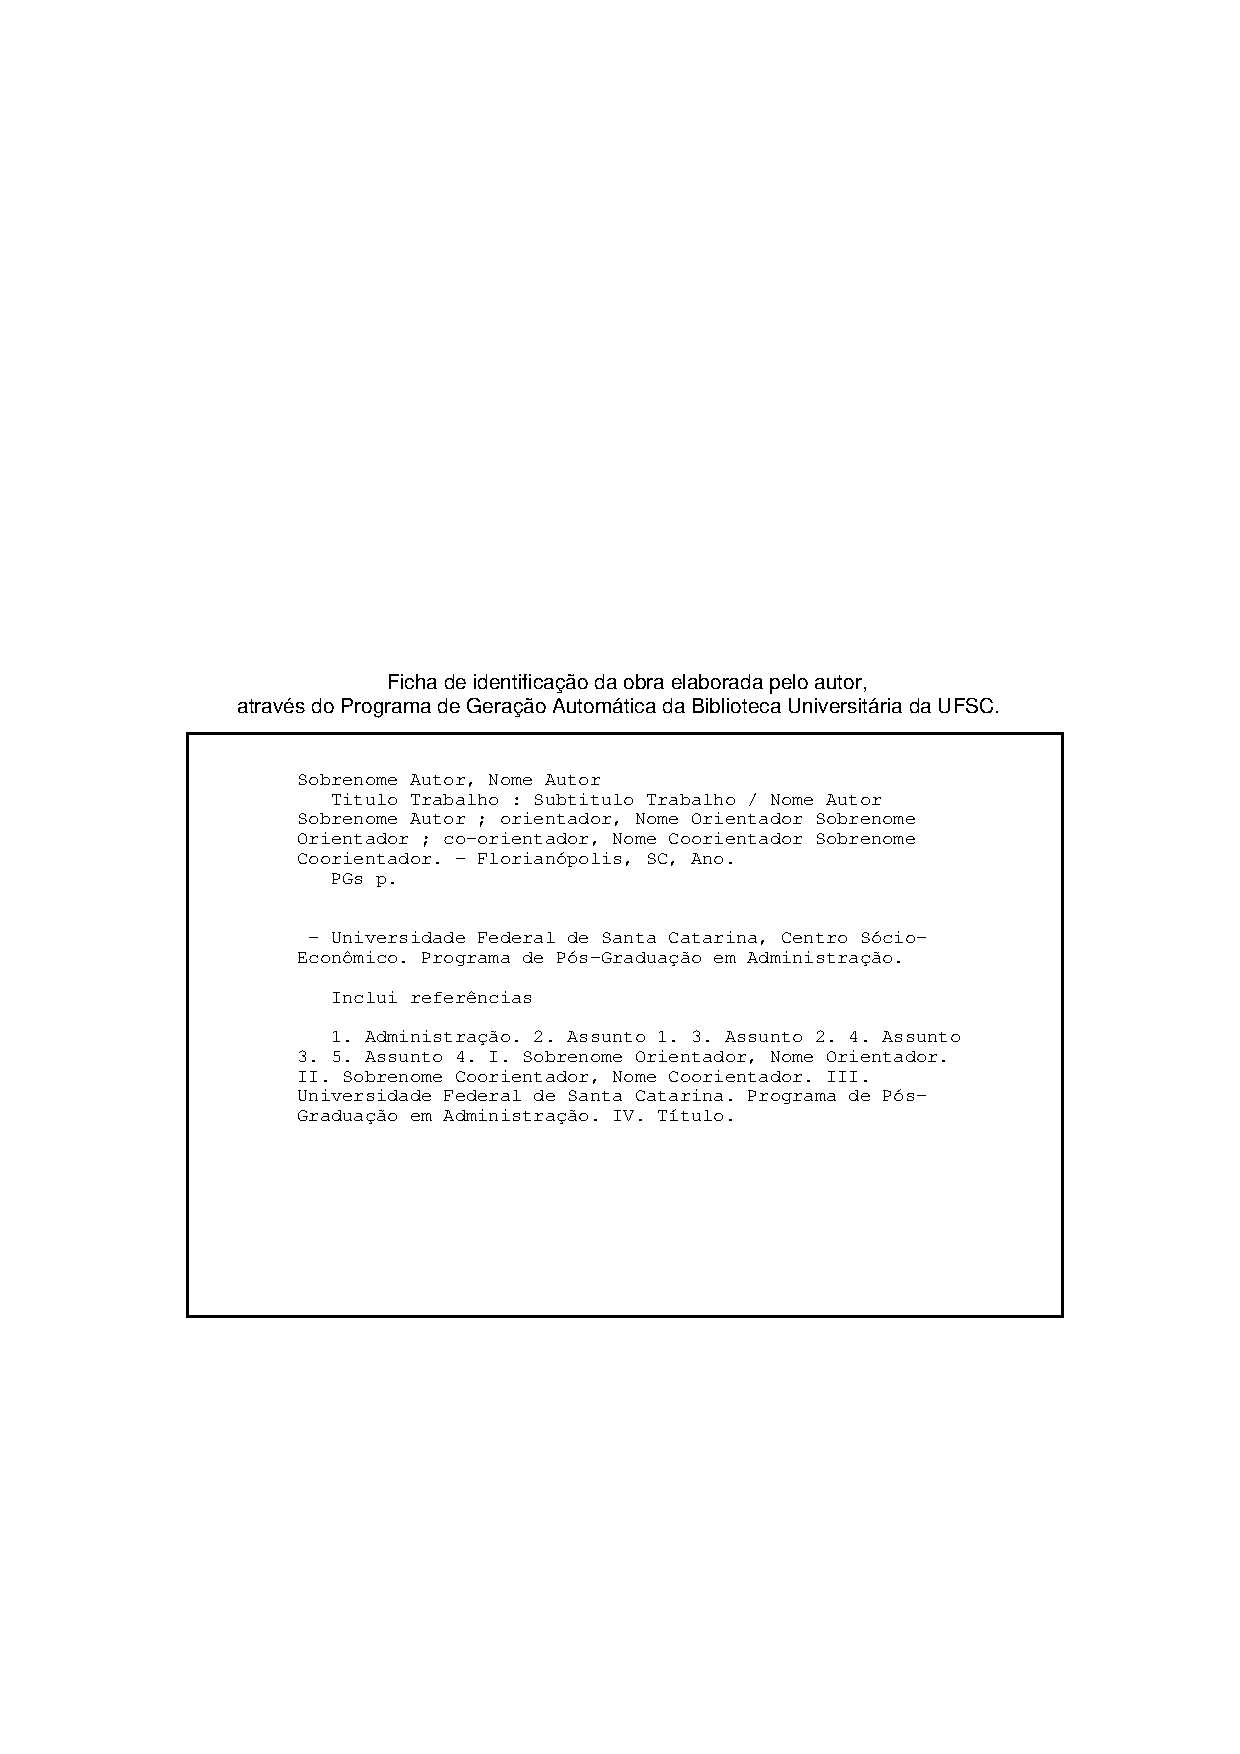
\includepdf{Ficha_Catalografica.pdf}
\end{fichacatalografica}

% \imprimirfichacatalografica%

% ---


% ---

% ---
% Inserir folha de aprovação
% ---

% Isto é um exemplo de Folha de aprovação, elemento obrigatório da NBR
% 14724/2011 (seção 4.2.1.3). Você pode utilizar este modelo até a aprovação
% do trabalho. Após isso, substitua todo o conteúdo deste arquivo por uma
% imagem da página assinada pela banca com o comando abaixo:
%
% \includepdf{folhadeaprovacao_final.pdf}
%
\begin{folhadeaprovacao}

	\begin{center}
		{\ABNTEXchapterfont\large\imprimirautor}
		
		\vspace*{\fill}
		\begin{center}
			\ABNTEXchapterfont\bfseries\Large\imprimirtitulo
		\end{center}
		\vspace*{\fill}

		\hspace{.45\textwidth}
		% \begin{minipage}{.5\textwidth}
		%     \imprimirpreambulo
		% \end{minipage}%
		\vspace*{\fill}
	\end{center}

	Este Trabalho de Conclusão de Curso foi julgado adequado para obtenção do 
	Título de ``Bacharel em Ciência da Computação'' e aprovado em sua forma final
	pelo Curso de Bacharelado em Ciência da Computação.
   
	\begin{center}   
	\imprimirlocal, 27 de novembro de 2018.
	\end{center}
	\assinatura{\textbf{Prof. Dr. Renato Cislagh} \\ Coordenador} 


	\noindent\textbf{\\Banca examinadora:}

	\assinatura{\textbf{\imprimirorientador} \\ 
		Orientador \\ Universidade Federal de Santa Catarina} 
	\assinatura{\textbf{Prof. Dr. Frank Augusto Siqueira} \\ Universidade Federal de Santa Catarina}
	\assinatura{\textbf{Prof.ª Dr.ª Patrícia Della Méa Plentz} \\ Universidade Federal de Santa Catarina}
  
\end{folhadeaprovacao}
% ---

% ---
% Dedicatória
% ---
\begin{dedicatoria}
   \vspace*{\fill}
   \centering
   \noindent
   \todo[inline]{\textit{ Este trabalho é dedicado à...}} \vspace*{\fill}
\end{dedicatoria}
% ---

% ---
% Agradecimentos
% ---
\begin{agradecimentos}
	\todo[inline]{ToDo}
\end{agradecimentos}
% ---

% ---
% Epígrafe
% ---
\begin{epigrafe}
    \vspace*{\fill}
	\begin{flushright}
		\todo[inline]{\textit{ToDo}}
		\textit{``Some citation''\\
		(Surname, Name)}
	\end{flushright}
\end{epigrafe}
% ---

% ---
% RESUMOS
% ---


% resumo em português
\setlength{\absparsep}{18pt} % ajusta o espaçamento dos parágrafos do resumo
\begin{resumo}
	Uma nova classe de \emph{chips} altamente paralelos de baixo consumo energéitco que lidam com a restrição de energia foram descobertos. Os processadores Sunway SW26010 e Kalray MPPA-256 são exemplos deles, entregando mais de duzentos núcleos de processamento em um único \emph{chip} de baixo consumo energético. Apesar de apresentarem melhor eficiência energética do que os processadores \emph{multicore} de propósito geral, características arquiteturais como a limitada quantidade de memória ditribuída no \emph{chip} torna o desenvolvimento de aplicações científicas paralelas eficientes uma tarefa desafiadora. Neste projeto foram propostas otimizações ao \fw PSkelMPPA, que prove uma abstração única e de alto nível para programação estêncil no processador \mppa, livrando os programadores de serem responsáveis pela tarefa de explicitamente lidar com a comunicação e com o modelo de programação paralela híbrida do \mppa.

	\textbf{Palavras-chave}: \Manycore. \mppa. Processamento de alto desempenho. Eficiência energética.
\end{resumo}

% resumo em inglês
\begin{resumo}[Abstract]
	\begin{otherlanguage*}{english}
		\todo[inline]{ToDo}

   		\vspace{\onelineskip}
 
   \noindent 
   \textbf{Keywords}: ToDo.
 \end{otherlanguage*}
\end{resumo}



% ---
% inserir lista de ilustrações
% ---
\pdfbookmark[0]{\listfigurename}{lof}
\listoffigures*
\cleardoublepage
% ---

% ---
% inserir lista de tabelas
% ---
% \pdfbookmark[0]{\listtablename}{lot}
% \listoftables*
% \cleardoublepage
% ---

% ---
% inserir lista de abreviaturas e siglas
% ---
\begin{siglas}
  \item[\mppa] \textit{Massively Parallel Processor Array}
  \item[\io] Entrada e Saída
  \item[\noc] \textit{Network-on-Chip}
  \item[\cpu] \textit{Central processing unit}
  \item[\gpu] \textit{Graphics processing unit}
  \item[\api] \textit{Application Programming Interface}
  \item[\ipc] \textit{Inter-Process Communication}
\end{siglas}
% ---

% ---
% inserir lista de símbolos
% ---
% \begin{simbolos}
%   \item[$ \Gamma $] Letra grega Gama
%   \item[$ \Lambda $] Lambda
%   \item[$ \zeta $] Letra grega minúscula zeta
%   \item[$ \in $] Pertence
% \end{simbolos}
% ---

% ---
% inserir o sumario
% ---
\pdfbookmark[0]{\contentsname}{toc}
\tableofcontents*
\cleardoublepage
% ---



% ----------------------------------------------------------
% ELEMENTOS TEXTUAIS
% ----------------------------------------------------------
\textual

% ----------------------------------------------------------
% Introdução
% ----------------------------------------------------------
\chapter[Introdução]{Introdução}

Até a última década, o desempenho das arquiteturas utilizadas na área de Computação de Alto Desempenho (\textit{High Performance Computing} - HPC) tem sido quase exclusivamente quantificado pelo seu poder de processamento. No entanto, a eficiência energética está sendo considerada recentemente tão importante quanto o desempenho e tornou-se um aspecto crítico para o desenvolvimento de sistemas escaláveis~\cite{francesquini:hal-01092325}. Portanto a pesquisa e o desenvolvimento científico nesta área com enfoque na redução do consumo de energia tem se tornado de extrema importância para o avanço tecnológico.

Assim, é notório o surgimento de uma nova classe de processadores, os denominados processadores \textit{manycore}, com mais de centenas de núcleos de processamento e de baixo consumo de energia, capazes de lidar com o paralelismo dados e tarefas, como o \mppa~\cite{castro2013}. 
Apesar dos benefícios oriundos dos processadores \textit{manycore}, eles também trazem desafios para a programação de aplicações paralelas devido às suas características arquiteturais~\cite{castro:hal-01273153}. Uma das formas de simplificar o desenvolvimento de aplicações paralelas, abstraindo os detalhes arquiteturais e de programação de baixo nível, é através da utilização de padrões paralelos ou esqueletos algorítimicos~\cite{COLE2004389}.

Um destes padrões é denominado estêncil. Este padrão consiste em varrer os elementos de um dado \textit{array} de entrada de \textit{n}-dimensões, e modificar o valor de cada elemento com base nos valores dos elementos vizinhos, produzindo assim um \textit{array} de saída de \textit{n}-dimensões com valores modificados. Além disso, essa etapa de varredura e modificação de valores pode ser realizada iterativamente, na qual o \textit{array} de saída de uma iteração, será o \textit{array} de entrada da iteração seguinte. É válido destacar que muitos destes padrões estão presentes nas mais diversas áreas do conhecimento, como física, matemática, processamento de imagens, entre outros~\cite{Holewinski:2012:HCG:2304576.2304619}.

Dentre os \fws propostos, o \pskel se destaca por prover uma abstração para ambientes heterogêneos de programação, que contam com a presença de processadores \textit{multicore} e placas gráficas. Além disso, foram observados ganhos na performace média de até 76\%~\cite{CPE:CPE3479}.

Com a necessidade e importância de cunho científico do desenvolvimento de aplicações paralelas nos processadores \textit{manycore}, foi proposta uma adaptação do \textit{framework} \pskel para que ele dê suporte ao processador \mppa. Os resultados obtidos com o \pskel no \mppa foram promissores, apresentando uma redução no consumo energético de aplicações estêncil quando comparado  com execuções em um processador de alto desempenho Intel Broadwell~\cite{wscad2017}.

Todavia, foi observado que o tempo desperdiçado na comunicação das aplicações do \mppa é elevado e impacta diretamente nos testes e experimentos realizados, comunicação está que ocorre através de \textit{Networks-on-Chip} (NoCs) de dados e de controle. Decorrente desta estrutura, o delay de comunicação entre elementos fisicamente mais distantes na rede será maior do que elementos mais próximos.

Além disso, a atual API de comunicação utilizada no \pskel para o \mppa é similar ao modelo clássico POSIX de baixo nível para \textit{Inter-Process Communication} (IPC), o que dificulta o desenvolvimento de rotinas de comunicação e expõe essas rotinas a possíveis perdas de desempenho não trivialmente detectáveis. A nova API de comunicação assíncrona desenvolvida e disponibilizada pelos desenvolvedores do processador, eleva o nível de abstração dessas rotinas de comunicação com implementações otimizadas para o processador, acarretando em maior robustez e desempenho na utilização da NoC. Com isso, nota-se a importância da revisão e estudo da implementação atual da adaptação do \textit{framework} \pskel para o \mppa, visando encontrar espaços para otimização e ganho de desempenho, que impactarão diretamente no gasto energético do processador, que já se mostrou promissor quando comparado ao Intel Broadwell. 
% ---------------------------------

% ---------------------------------
\section{Objetivos}
\label{sec:objetivos}
A medida que se reduz o número de comunicações e sincronizações, através do aumento do número de elementos processados a cada iteração de uma aplicação de computação estêncil no \mppa é observada a queda no tempo de sua execução e por consequência a redução do consumo de energia~\cite{wscad2017}.

\subsection{Objetivos Gerais}
\label{subsec:objetivos-gerais}

 Portanto, uma vez identificado que os gastos de comunicação são fatores relevantes para a influência do consumo de energia e tempo de execução das aplicações, este \textit{Trabalho de Conclusão de Curso} tem como objetivo geral propor otimizações na comunicação de dados para o \fw \pskel adaptado para o \mppa visando o ganho de desempenho e redução de consumo de energia pelas aplicações paralelas de padrão estêncil no \mppa.

\subsection{Objetivos Especificos}
\label{subsec:objetivos-específicos}

Os objetivos específicos deste trabalho são: 

\begin{enumerate}
\item Estudar a nova API de comunicação assíncrona disponibilizada pelo fabricante do processador e realizar as modificações de código necessárias no \pskel para fazer uso da mesma;
\item Propor e implementar otimizações na comunicação e na distribuição de dados entre os elementos de processamento a fim de se obter ganhos de desempenho e redução no consumo de energia;
\item Realizar experimentos com aplicações estêncil para medir o desempenho e a eficiência energética das otimizações propostas, comparando resultados obtidos com outros processadores \textit{multicore} e processadores gráficos.
\end{enumerate}

% ----------------------------------------------------------
% Fundamentação Teórica
% ----------------------------------------------------------
\chapter[Fundamentação Teórica]{Fundamentação Teórica}


% ----------------------------------------------------------
% Trabalhos relacionados
% ----------------------------------------------------------
\chapter[Trabalhos Relacionados]{Trabalhos Relacionados}


\section{Trabalhos Relacionados}

Devido a importância dos esqueletos paralelos, e especifcamente o padrão paralelo estêncil, muitos esforços de pesquisas recentes buscam melhorar o desempenho e o suporte desses esqueletos em processadores manycore. \textit{Buono}~\cite{buono13} portou um \fw baseado em esqueletos paralelos, chamado \textit{FastFlow}, para o processador \textit{manycore} TilePro64, que possui 64 núcleos de processamento idênticos, interconectados por uma malha de \noc. Similarmente,~\cite{thoraransen16} apresentou um novo \textit{back-end} do \fw SkePU para o processador \textit{manycore} Myriad2. Que possui como característica uma arquitetura heterogenea, visando dispositivos com restrição de energia e principalmente aplicações de visão computacional. \textit{Gysi}~\cite{gysi15} propôs um \fw para otimização automática da repartição de computações estêncil em sistemas híbridos de \cpu e \gpu.

Recentes trabalhos estudaram o desempenho e/ou a eficiência energética de processadores manycore de baixa potência. \textit{Totoni}~\cite{SCCEnergy:2012} comparou a potência e o desempenho do \textit{Intel's Single-Chip Cloud Computer} (SCC) com outros tipos de \textit{CPUs} e \textit{GPUs}. Porém, eles mostraram que não existe um solução única que entrega o melhor troca entre potência e performance, os resultados mostram que \textit{manycores} são uma oportunidade para o futuro. \textit{Souza}~\cite{Castro-Souza-CCPE:2016} propôs um conjunto de \textit{benchmarks} para avaliar o \mppa manycore processor. O \textit{benchmark} oferece diversas aplicações que utilizam padrões paralelos, tipos de trabalho, intensidade de comunicação e estratégias de carga de trabalho, adequado para uma ampla compreensão do desempenho e consumo de energia do \mppa e novos \textit{manycores} que estão por vir. \textit{Francesquini}~\cite{Castro-IA3-JPDC:2014} avaliou três diferentes classes de aplicação (consumo de CPU, consumo de memória e uma composição híbrida dos dois tipos anteriores) utilizando plataformas de alto paralelismo como o \mppa em uma plataforma NUMA de 24 nós e 192 núcleos. Eles mostraram que as arquiteturas \textit{manycore} podem ser competitivas, mesmo se a aplicação é irregular por natureza.

De acordo com relevante conhecimento na área, o \pskelmppa é a primeira implementação completa de um \fw com uso de padrões paralelos no \mppa. A solução proposta livra os programadores da necessidade de lidar explicitamente com a gestão de comunicação e envio de dados pela \noc, assim como a preocupação de lidar com um ambiente híbrido de execução e a ausência de coerência de cache no \mppa.

% ----------------------------------------------------------
% Otimização PSkel-MPPA
% ----------------------------------------------------------
% \chapter[Otimização PSkel-MPPA]{Otimização PSkel-MPPA}


% ----------------------------------------------------------
% Experimento
% ----------------------------------------------------------
% \chapter[Experimentos]{Experimentos}



% ----------------------------------------------------------
% Finaliza a parte no bookmark do PDF
% para que se inicie o bookmark na raiz
% e adiciona espaço de parte no Sumário
% ----------------------------------------------------------
\phantompart

% ----------------------------------------------------------
% Conclusão
% ----------------------------------------------------------
% \chapter[Conclusão]{Conclusão}



% ----------------------------------------------------------
% ELEMENTOS PÓS-TEXTUAIS
% ----------------------------------------------------------
\postextual
% ----------------------------------------------------------

% ----------------------------------------------------------
% Referências bibliográficas
% ----------------------------------------------------------
\bibliography{bibliografia}

% ----------------------------------------------------------
% Glossário
% ----------------------------------------------------------
%
% Consulte o manual da classe abntex2 para orientações sobre o glossário.
%
%\glossary

% ----------------------------------------------------------
% Apêndices
% ----------------------------------------------------------

% ---
% Inicia os apêndices
% ---
\begin{apendicesenv}

% Imprime uma página indicando o início dos apêndices
\partapendices

% ----------------------------------------------------------
% Apêndice A
% ----------------------------------------------------------
% \chapter{}

\end{apendicesenv}
% ---


% ----------------------------------------------------------
% Anexos
% ----------------------------------------------------------

% ---
% Inicia os anexos
% ---
\begin{anexosenv}

% Imprime uma página indicando o início dos anexos
\partanexos

% ----------------------------------------------------------
% Anexo A
% ----------------------------------------------------------
% \chapter{}


\end{anexosenv}

%---------------------------------------------------------------------
% INDICE REMISSIVO
%---------------------------------------------------------------------
\phantompart
\printindex
%---------------------------------------------------------------------

\end{document}
